\section{Introduction}

Difference-in-differences (DID) is among the most widely used methods for causal inference in non-experimental settings. In many applications, however, compliance is imperfect. Some units in the treated group do not take up treatment, and some in the control group do \citep[e.g.,][]{duflo2001schooling, cornelissen2018benefits, kennedy2023hidden}. In such \textit{fuzzy} designs, the standard DID estimand recovers only an intention-to-treat effect, which is known to understate the effects among the treated. \cite{fuzzy2018} show that the Wald-DID ratio, i.e.\ the DID in outcomes divided by the DID in treatment take-up, identifies a local average treatment effect (LATE) under monotonicity and treatment-effect stability, and propose a Time-Corrected (TC) variant that relaxes stability by using within-status outcome trends in the control group.

In order to relax identification assumptions, both Wald-DID and TC estimands can be extended to accommodate covariates. In modern applications the relevant covariate set can be high-dimensional, with the number of covariates potentially much larger than the sample size. Machine learning methods handle high dimensions through regularization, but the resulting first-step bias introduced by this type of learner contaminates plug-in treatment-effect estimators \citep{DDML2018}.

This paper develops debiased machine learning (DML) estimators for the Wald-DID and Time-Corrected estimands. I recast both estimands as unconditional moment restrictions and derive orthogonal scores for each using the first-step influence function approach of \citet{ichimura2022influence}. The resulting scores are locally robust in the sense of \citet{chernozhukov2022locally} and satisfy Neyman orthogonality. The cross-fitted GMM estimators built from them are $\sqrt{n}$-consistent and asymptotically normal under the standard $n^{-1/4}$ product-rate condition on the first-step nuisance estimates (Theorem~\ref{thm:1}). The orthogonal scores are proportional to the efficient influence functions of the two estimands, so the cross-fitted GMM estimators attain the semiparametric efficiency bound (Proposition~\ref{prop:4}). The framework accommodates flexible first-step learners, including Lasso, random forests, and neural networks.

\begin{figure}[H]
    \centering
    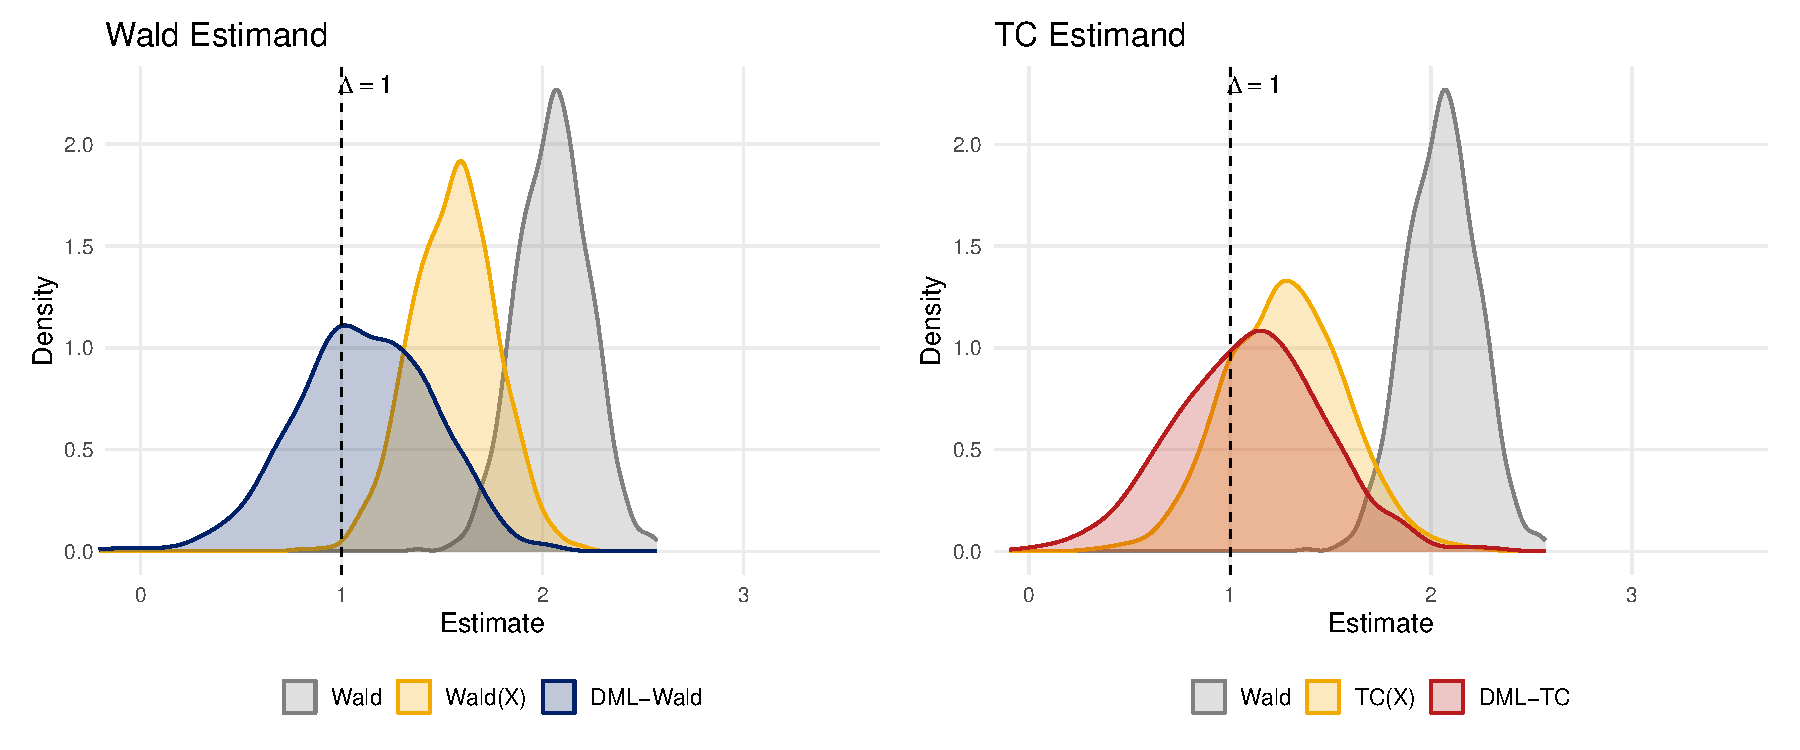
\includegraphics[width=\linewidth]{../output/figures/fig1_production.pdf}
    \caption[Sampling distribution of estimators]{Sampling distribution of estimators (true $\Delta=1$, dashed line; $n=5{,}000$, $p=100$ with 20 signal $+$ 80 noise, $M=1{,}000$). Left: Wald estimand. Right: TC estimand. The Wald estimator without covariates (grey, baseline in both panels) is consistent but noisy. The Lasso plug-in estimators (Wald$_X$, TC$_X$; gold) exhibit bias equal to 56\% and 28\% of the true effect. The DML estimators (DML-Wald in blue, DML-TC in red) reduce bias to 11\% and 10\%, attain 90--95\% coverage, and are centered near the truth.}\label{fig:1}
\end{figure}

A second contribution is a data-driven trimming algorithm for the propensity score. The proposed DML scores involve inverse-probability weights that become unstable when the probability of belonging to the treated group approaches one. Extending \cite{crump2009trimming} from the average treatment effect to our DID-IV estimands, I propose a data-driven, one-sided trimming rule that targets a sample analog of the estimator's asymptotic variance. The rule excludes only observations with high treatment probability, imposes no lower bound, and does not require knowledge of the true treatment effect. Monte Carlo simulations show it reduces variance and RMSE relative to fixed symmetric thresholds, at the cost of some bias because the trimmed estimand is not exactly the LATE. Appendix~\ref{sec:app_trimming} states formal optimality as a conjecture and derives the one-sided form under homoskedasticity and a weak monotonicity condition on the conditional first stage.

Monte Carlo simulations with $M=1{,}000$ replications confirm that DML-Wald and DML-TC attain near-nominal coverage at moderate sample sizes (Figure~\ref{fig:1}), while Lasso plug-in alternatives undercover by 17 to 46 percentage points. An application to the INPRES school construction program in Indonesia \citep{duflo2001schooling} uses a $p = 45$ individual-level dictionary and illustrates both contributions. Relative to the Lasso plug-in, the DML correction shifts point estimates downward across specifications and tightens cluster-robust confidence intervals at the primary-completion margin, and the trimming algorithm certifies common support when the propensity distribution stays interior.

The rest of the paper is organized as follows. Section~\ref{sec:lit} reviews the related literature. Section~\ref{sec:2} describes the Wald-DID and TC estimands. Section~\ref{sec:3} develops the locally robust estimators and states Theorem~\ref{thm:1}. Section~\ref{sec:4} presents the propensity score trimming algorithm. Section~\ref{sec:5} presents Monte Carlo evidence. Section~\ref{sec:6} applies the estimators to INPRES. Section~\ref{sec:7} concludes.
